\newpage
\subsection{The shutter system}
\label{shutter}
The shutter system is a sub-system allowing the microcontroller to command the camera. This system was developed with the help of video tutorials dismantling commercial remote shutters, showing that they were mainly made of resistances.
%Schematic of the shutter system
\begin{figure}[!h]
    \centering
    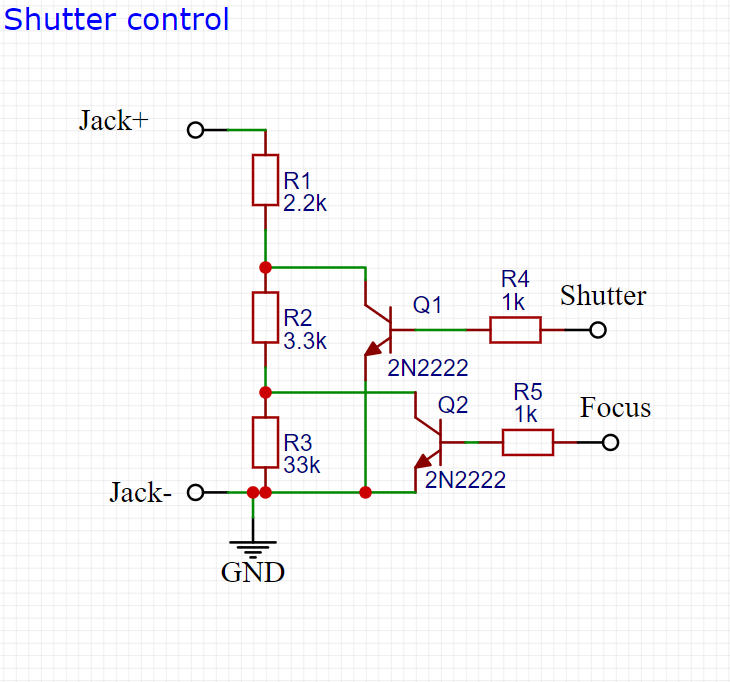
\includegraphics[width=0.7\textwidth]{\currfiledir/figures/shutter.png}
    \caption{Schematic of the shutter system}
    \cite{JACK}
\end{figure}

\begin{figure}[!h]
    \centering
    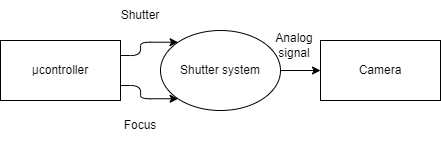
\includegraphics[width=0.9\textwidth]{\currfiledir/figures/shutter_diagram.png}
    \caption{Shutter system}
\end{figure}

The system is made of a jack socket, connected to resistances. The shutter and the focus pin are linked to the microcontroller. The microcontroller can then be programmed to put the pins at a high or a low state to trigger the shutter or the focus of the camera. By controlling transistor, the camera sees a change in the resistor and trigger the associated actions.